\section{findplace?}
Hsing et al.\cite{hsing2008use} reportThey found gene ontology terms to be useful classifiers and found `RNA binding',`translation' and `ribosome' highly represented. I have used the top and bottom 10th centile\footnote{mainly because this generates sets of around 345 genes which are more easily interpretable in over representation analysis and that the top 10\% of values are markedly more extreme}.

The literature has often shown that loss of function in hubs are lethal \cite{jeong2001lethality} however more recent results suggest the situation may be complex (see section~\ref{sec:Degree and essentialness}) and some argue that hub changes lead to more to pleiotropy\cite{yu2008high}. Yeast hub nodes were found to be more evolutionarily ancient and had higher number of multiple and repeated domains\cite{ekman2006properties} and previous work suggests genes related to intelligence are in evolutionarily conserved regions\cite{hill2016molecular}. 

\section{Extra from gene ontology enrichment}
% latex table generated in R 3.6.3 by xtable 1.8-4 package
% Sun Oct  4 15:30:52 2020


% latex table generated in R 3.6.3 by xtable 1.8-4 package



across all of theGene ontology enrichment of the most central vertices reveals that they share a number of common properties across different





\subsection{Moved from other sections}
\paragraph{Results GO enrichment Closeness}
More normally distributed.
High closeness RNA binding, severe murine phenotype, cellular component cell adhesion
Ca and neurodegenerative

Low closeness centrality transporter activity, seizures in human phenotype, receptor activation, disease top five all epilepsies. 

\subsection{Degree}
High degree nodes are enriched for terms associated with RNA binding, cell cycle and ubiquitin binding. This would be consistent with these high degree nodes being involved in central cellular processes\footnote{\url{source('~/RProjects/chapter3/R/sig_magma_genes/central_genes_ToppGene/degree/5_0_clip_centrality_degree_high_mf_n_10.R')}}.

\paragraph{Molecular function}
Molecular function table~\ref{tab:ToppGENE GO: Molecular Function. 90 centile cwpsp.txtp = p value; q FDR B H = q adjusted significance level False Discovery Rate using Benjamini and Hochberg adjustment; n= n genes annotated in test group; n PSP= n genes annotated in PSP. n significant in category 186} shows enrichment for ubiquitin protein ligase, RNA binding and transcription factor binding. The q values are not as significant as those for kcoreness and eigenvector centrality.

% latex table generated in R 3.6.3 by xtable 1.8-4 package
% Sun Oct  4 15:28:01 2020





\clearpage
\begin{figure}
    \centering
    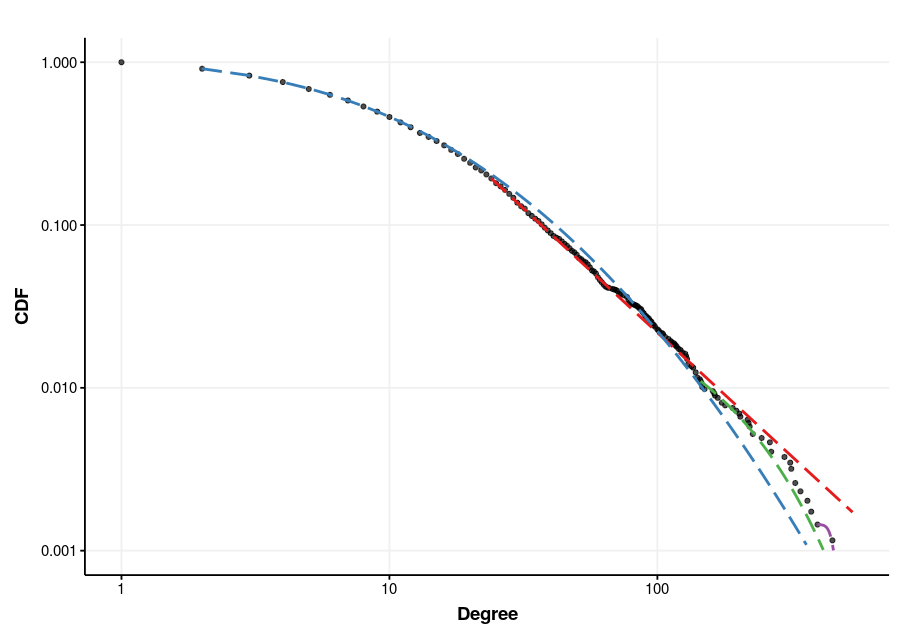
\includegraphics[width=\textwidth]{images/chapter3/poweRlaw/RPlot_plot_powerlaw_xmin_set_for_each_distribution_add_theme.png}
    \caption{FIT OVER ALL CDF of degree distribution and lines of best fit for power law (red), log-normal(blue) exponential(green) and poisson (purple). Poisson distribution is clearly a poor fit with x min close to x max (396) and the exponential distribution holds only in x min greater than 145. x axis degree log 10 scaled, y axis CDF log 10 scaled. Exponential appears a good fit but is fitted to a much smaller part of the distribution than the power law and log-normal. Poisson distribution is clearly not a good fit.} 
    \small\url{source('~/RProjects/chapter3/R/fit_power_law/graphing/plot_power_law_and_lognormal_ggplot2_add_theme.R')}
    \label{fig:CDF degreel_theme}
\end{figure}



% bootstrap p log-normal 0.4
\begin{figure}
    \centering
    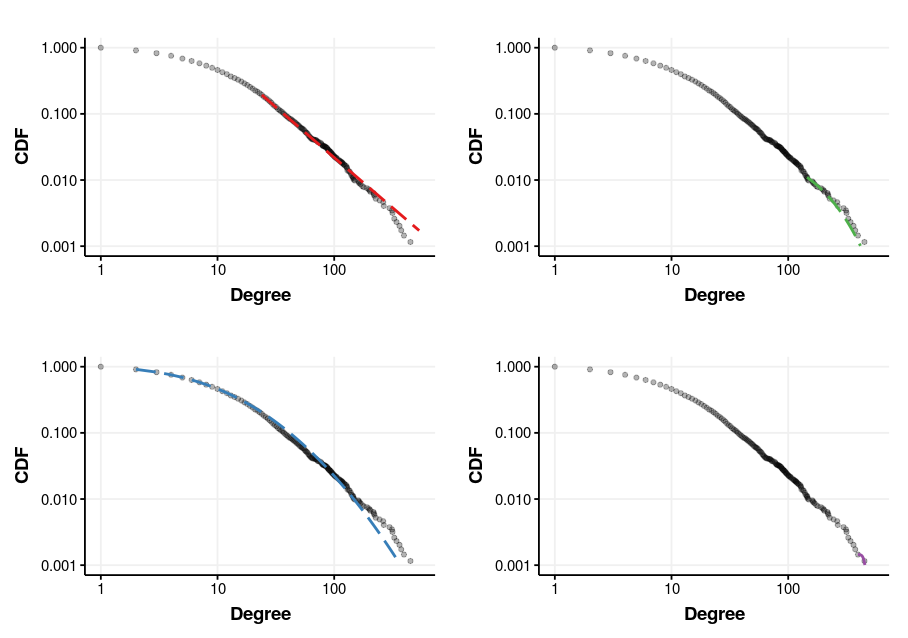
\includegraphics[width=\textwidth]{images/chapter3/poweRlaw/multiplot/Rplot_multiplot_with_x_min_each_distribution.png}
    \caption{FIT OVER ALL CDF of degree distribution and lines of best fit for power law (red), log-normal(blue) exponential(green) and poisson (purple). Poisson distribution is clearly a poor fit with x min close to x max (396) and the exponential distribution holds only in x min greater than 145. x axis degree log 10 scaled, y axis CDF log 10 scaled. Exponential appears a good fit but is fitted to a much smaller part of the distribution than the power law and log-normal. Poisson distribution is clearly not a good fit.}
    \small\url{source('~/RProjects/chapter3/R/fit_power_law/graphing/plot_power_law_and_lognormal_ggplot2_multiplot.R')}
    \label{fig:CDF degreel_multiplot}
\end{figure}
% p exponential < 0.01
